\phantomsection
\chapter{Feature extraction}
\label{chap:extraction}

\noindent After having detected the face, for example using Viola-Jones algorithm, it is necessary to perform feature extraction in order to process data before classification. 
This step takes an image as input, and extracts vectors characterizing its main features. In the case of a facial expression recognition system, resulting vectors contain informations about spacial configuration of facial features, but can also encode informations about shape, texture or movement of the image's content \cite{CHI03}.
\newline

\noindent There are however many kinds of algorithms outputting features vectors, and the choice of an effective one depends on many criteria. These feature extraction methods can generally be ranked among 2 categories: they can either be appearance-based or feature-based, depending on the way they extract feature vectors. The aim of this chapter is to explain the differences between these 2 types of feature extraction methods, and provide some examples from each category.
\newline

\vspace{\baselineskip}
\noindent Before developing a facial expression recognition project, it is important to know what already exists; the state of the art of facial expression recognition system. In this chapter, an overview will be given of the existing systems before to decide on a feature extraction system for the project.
\newline

\noindent Two main categories of feature extraction algorithms can be distinguished : \textit{appearance-based} or \textit{feature-based}. The first ones are algorithms that try to find basic vectors characterizing the whole picture, usually by a dimensionality reduction method. These algorithms lead to a simplification of the dataset, while retaining the main characteristics of the picture. However, these methods have to be carefully parametrized, so they do not encounter the "curse of dimensionality", which is about processing high-dimensional data.
\vspace{\baselineskip}

\noindent Examples of appearance-based methods : Principal Component Analysis, Linear Discriminant Analysis, Hidden Markov Models, Eigenfaces.
\newline

\noindent The second type of feature extraction algorithms are feature-based algorithms. These methods tend to locate important features, and build the feature vectors depending on those regions of interest. The key point of these methods is that the face is not a global structure anymore. Indeed, it has been summarized in a set of features regions, which are themselves translated into feature vectors.
\vspace{\baselineskip}

\noindent Examples of feature-based methods : Gabor Wavelets, Local Binary Patterns.
\newline

\vspace{\baselineskip}
\noindent Before developing a facial expression recognition project, it is important to know what already exists; the state of the art of facial expression recognition system. In this chapter, an overview will be given of the existing systems before to decide on a feature extraction system for the project.
\newline

\phantomsection
\section{Appearance-based methods}

\noindent As said in the introduction, the Appearance-based method aims to extract the appearance changes of the face. In order to do that the method uses image filters that are applied to the whole face or that are applied to specific parts of the face \cite{SHA09}. With this kind of method, if there is any change in the lighting or the pose of the head, the recognition will be less effective.
\newline

\subsection{Principal Component Analysis (PCA)}

\vspace{\baselineskip}
\noindent This is a statistical method; one of the most used in linear algebra. PCA is mainly used to reduce high dimensionality of data and to obtain the most important information out of it. PCA computes a covariance matrix and a set of values called the eigenvalues and eigenvectors from the original data \cite{GAN08}. Its output is a new coordinate system with lower dimensions, obtained from transformed high dimensionality of data, while preserving the most important information.  Since it is a statistical method, it can also be used in the classification step.
\newline

\subsection{Linear Discriminant Analysis (LDA)}

\vspace{\baselineskip}
\noindent Linear Discriminant Analysis is also a statistical method, used to classify a set of objects into groups. It is done by looking at a specific set of features describing the objects. LDA as PCA are used to establish a linear relationship between the dimensions of the data. LDA uses this relationship to model the differences into classes, while PCA does not take any differences into account in the linear relationship. The idea behind LDA  is to perform a linear transformation on the data to obtain a lower dimensional set of features \cite{GAN08}. \newline

\phantomsection
\section{Feature-based methods}
% Gabor wavelets, LBP

\noindent As said in the introduction, the feature-based method aims to locate important facial components. The shape and the location of these facial features are extracted from an face image and then are concatenated into a features vector. This features vector represents the geometry of the face \cite{SHA09}.
\newline

\noindent Compared to appearance-based method, the feature-based method has equal or better results. This was recently tested by Valstar et al. \cite{VAL05} \cite{VAL06}.
\newline

\subsection{Gabor Wavelets}

\vspace{\baselineskip}
\noindent The most used Feature-based method is the Gabor wavelets because of their performance. Gabor filters are applied in order to extract a set of Gabor wavelet coefficients. Filter responses are obtained when Gabor filters are convolved with face image (see figure~\ref{gabor_wavelets_example}). These representations of face display locality and orientation performance \cite{JEM09}. Indeed, gabor kernels represent features of the face and can be placed wherever if fits on the face and with whatever orientation. The disadvantage of this method is that it needs reliable and accurate feature detection and also tracking if necessary \cite{SHA09}. Another disadvantage of the Gabor feature extraction is processing time. This algorithm is very time-consuming, and dimensions of resulting vectors are very large \cite{PRA09}.
\newline

\begin{figure}[!h]
\begin{center}
\noindent 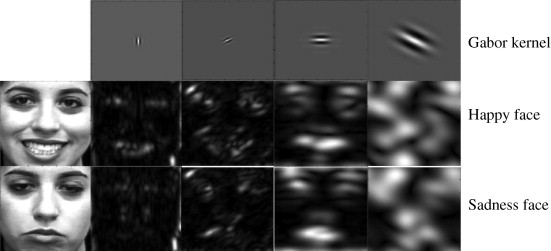
\includegraphics[scale=0.8]{figures/gabor_wavelets_example} 
\newline
\caption{Examples of Gabor wavelets and corresponding convoluted images}
\label{gabor_wavelets_example}
\end{center} 
\end{figure}

\subsection{Local Binary Patterns (LBP)}

\vspace{\baselineskip}
\noindent The Local Binary Pattern is a feature-based method. Its first application was to describe texture and shape of an image by extracting informations from the neighborhood of a central pixel. These informations are the output of the thresholding of intensity values from the neighborhood pixels with the intensity value of the central pixel \cite{GAN08}. One of the advantages of this method is that it is effective even when there is change in lighting (see figure~\ref{lbp_change_lighting}).
\newline

\begin{figure}[!h]
\begin{center}
\noindent 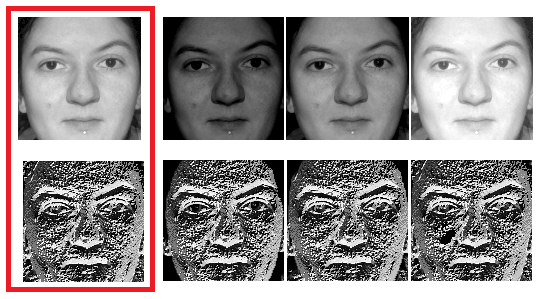
\includegraphics[scale=0.6]{figures/lbp_change_lighting} 
\newline
\caption{Effect of changes in lighting with LBP method}
\label{lbp_change_lighting}
\end{center} 
\end{figure}

\noindent This method is more detailed in Chapter \ref{chap:lbp}. This is this method that is used in this particular Facial Expression Recognition system. The choice has been made on this method because it is particularly effective and the implementation offers choices. This method was chosen over the Gabor wavelets one because the Gabor wavelets are known to be time consuming. And this Facial Expression Recognition system is wanted to be as close as possible of real-time system.
\newline

